\documentclass[%
  aps, reprint, prl, amsmath,amssymb
]{revtex4-2}

\usepackage{graphicx}% Include figure files
\graphicspath{{figures/}}
\usepackage{orcidlink}
\usepackage{mathtools}
\usepackage{algpseudocode}

% -------------- arXiv-Style Margin Stamp ----------------
\usepackage[style=iso]{datetime2}
\usepackage{FiraMono}
\usepackage{tikz}

% Use shipout/background to ensure it stays behind text/figures
\AddToHook{shipout/background}{
  \begin{tikzpicture}[remember picture, overlay]
    \node [
      rotate=90,
      color=gray!80,
      font=\fontfamily{FiraMono-TLF}\selectfont\footnotesize
    ] at ([xshift=1.2cm]current page.west) {
        WORKING DRAFT \quad $\bullet$ \quad \DTMnow \quad $\bullet$ \quad doi.org/10.17605/OSF.IO/EV8H6 \quad $\bullet$ \quad Brian S. Mulloy \quad $\bullet$ \quad bmulloy@umich.edu
    };
  \end{tikzpicture}
}
% --------------------------------------------------------

\begin{document}

\title{Symplectic Resolution of Semiclassical Singularities}

\begin{abstract}
\end{abstract}

\author{Brian S. Mulloy\orcidlink{0000-0002-1803-3172}}
\email{bmulloy@umich.edu}

\date{\today}

\maketitle

\section{The Quantum of Action}

\begin{figure}[t!]
    \centering
    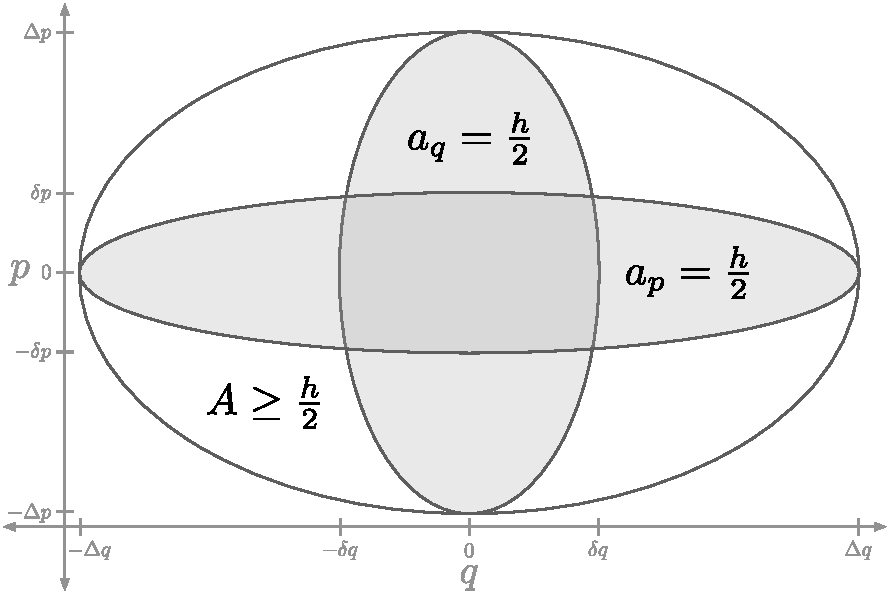
\includegraphics[width=\linewidth]{figures/quantum_of_action.png}
\caption{\textbf{The quantum of action} (schematic, 1D case). In symplectic geometry, the statistical Heisenberg limit, $\sigma_q \sigma_p \ge \hbar/2$, is characterized by classical semi-axes $\Delta q = \sqrt{2}\sigma_q$ and $\Delta p = \sqrt{2}\sigma_p$, establishing the relation $\pi \Delta q \Delta p \ge h/2$. In phase space, this defines the classical action area, $A \ge h/2$. The interior contains a conjugate pair of symplectic quantum blobs, $a_q = h/2$ and $a_p = h/2$, summing to the quantum of action, $h$. Specifically, $a_q$ is squeezed by the reciprocal boundary $\delta q = \hbar / \Delta p$ with an area of $\pi \delta q \Delta p = h/2$, while $a_p$ is constrained by the boundary $\delta p = \hbar / \Delta q$ with an area of $\pi \Delta q \delta p = h/2$. Together, these centered orthogonal ellipses enclose an interior ellipse with a quantum action area $a \le h/2$, given by $a = \pi \delta q \delta p = \pi \hbar^2/(\Delta q \Delta p)$. This inverse scaling geometrically enforces the correspondence principle: as the classical action area $A \ge h/2$ increases, the symplectic blobs $a_q$ and $a_p$ compress along their conjugate axes, shrinking the enclosed quantum action area $a$ (see Fig.~\ref{fig:qho_grid}). This symplectic hierarchy yields the quantum-classical relations $a = (\pi \hbar)^2 / A$ and $a \le h/2 \le A$.}
\label{fig:quantum_of_action}
\end{figure}

\begin{figure}[t!]
    \centering
    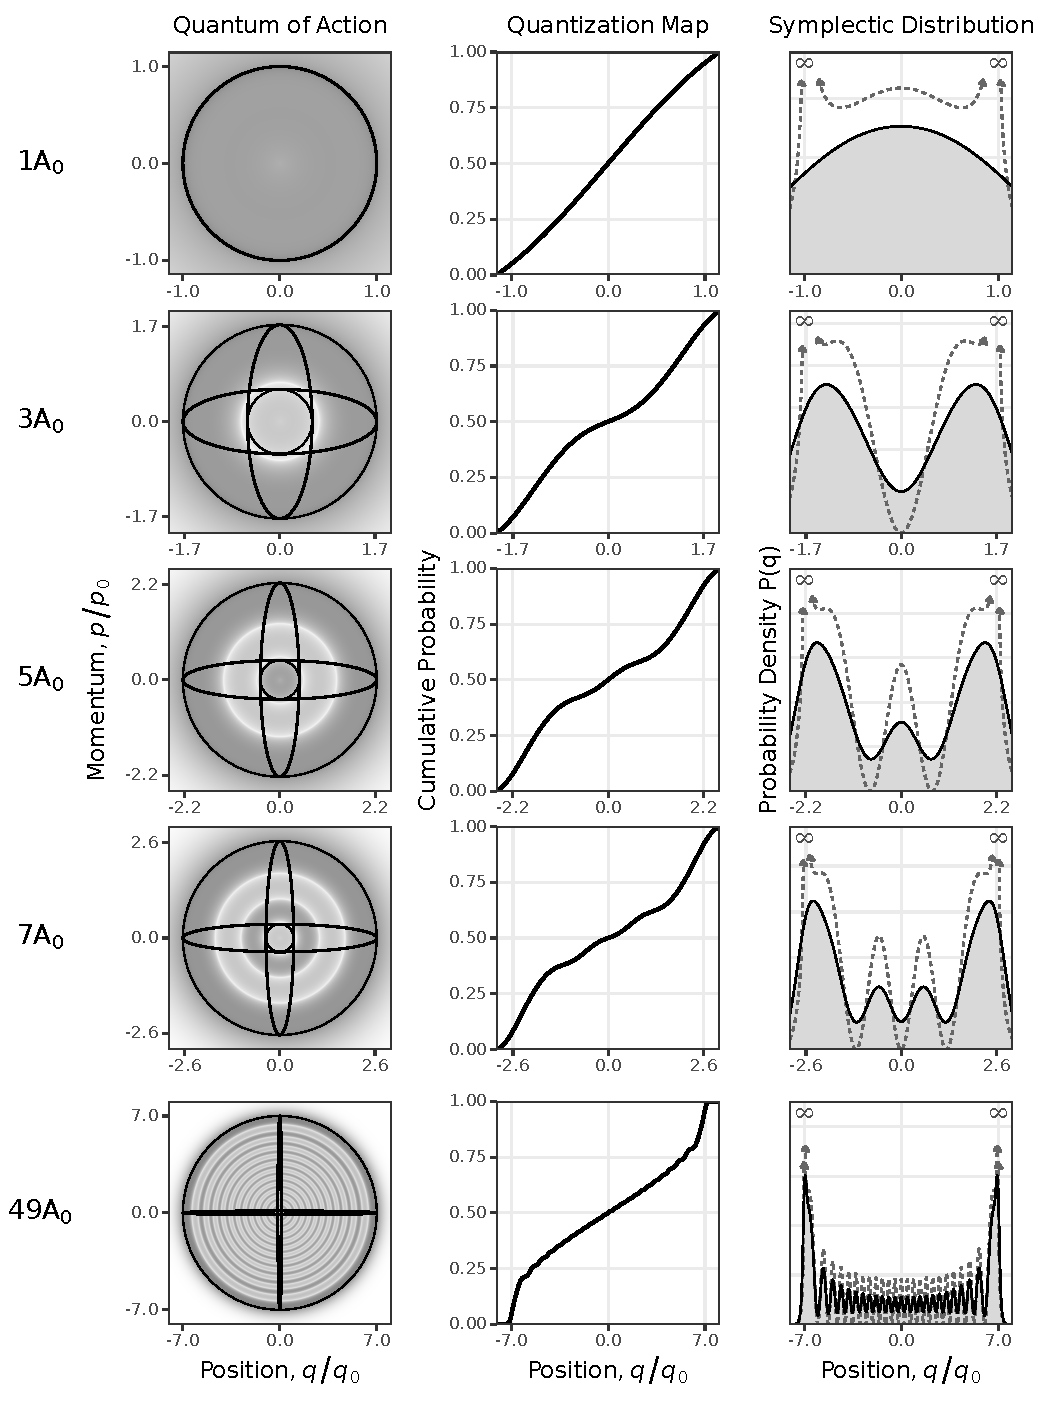
\includegraphics[width=\linewidth]{figures/qho_grid.png}
\caption{\textbf{Berry semiclassical quantum harmonic oscillator}.}
\label{fig:qho_grid}
\end{figure}

\bibliography{apssamp}

\end{document}
